%% This is an example first chapter.  You should put chapter/appendix that you
%% write into a separate file, and add a line \include{yourfilename} to
%% main.tex, where `yourfilename.tex' is the name of the chapter/appendix file.
%% You can process specific files by typing their names in at the 
%% \files=
%% prompt when you run the file main.tex through LaTeX.

\singlespacing{

\chapter{Simulation of Functional Digital Materials}\label{chap:functionSim}

Simulation of function-level parts is carried out through a mass/spring/damper model.  In this model, neighboring face-connected cells apply forces and torques on one another through local interactions.  Translational and rotational positions and velocities are calculated from these forces using discrete-time integration techniques.  Internal degrees of freedom of \textit{functions} are parameterized by 15 stiffness and damping coefficients, $k$ and $d$.  Actuation is achieved by modulating the nominal distance of adjacent cells along a particular degree of freedom.  %In a sense, this type of simulation could be thought of as a dynamic constraint-solving system between solid elements with various degrees of freedom.

\section{Existing Models of Solids}

Mass/spring/damper
FEA

%Unlike traditional mass/spring/damper models of solids from computer graphics literature (cite stuff here), the model developed in this thesis draws on an abstraction of the functionality embedded in the different "function types".

\begin{figure}
  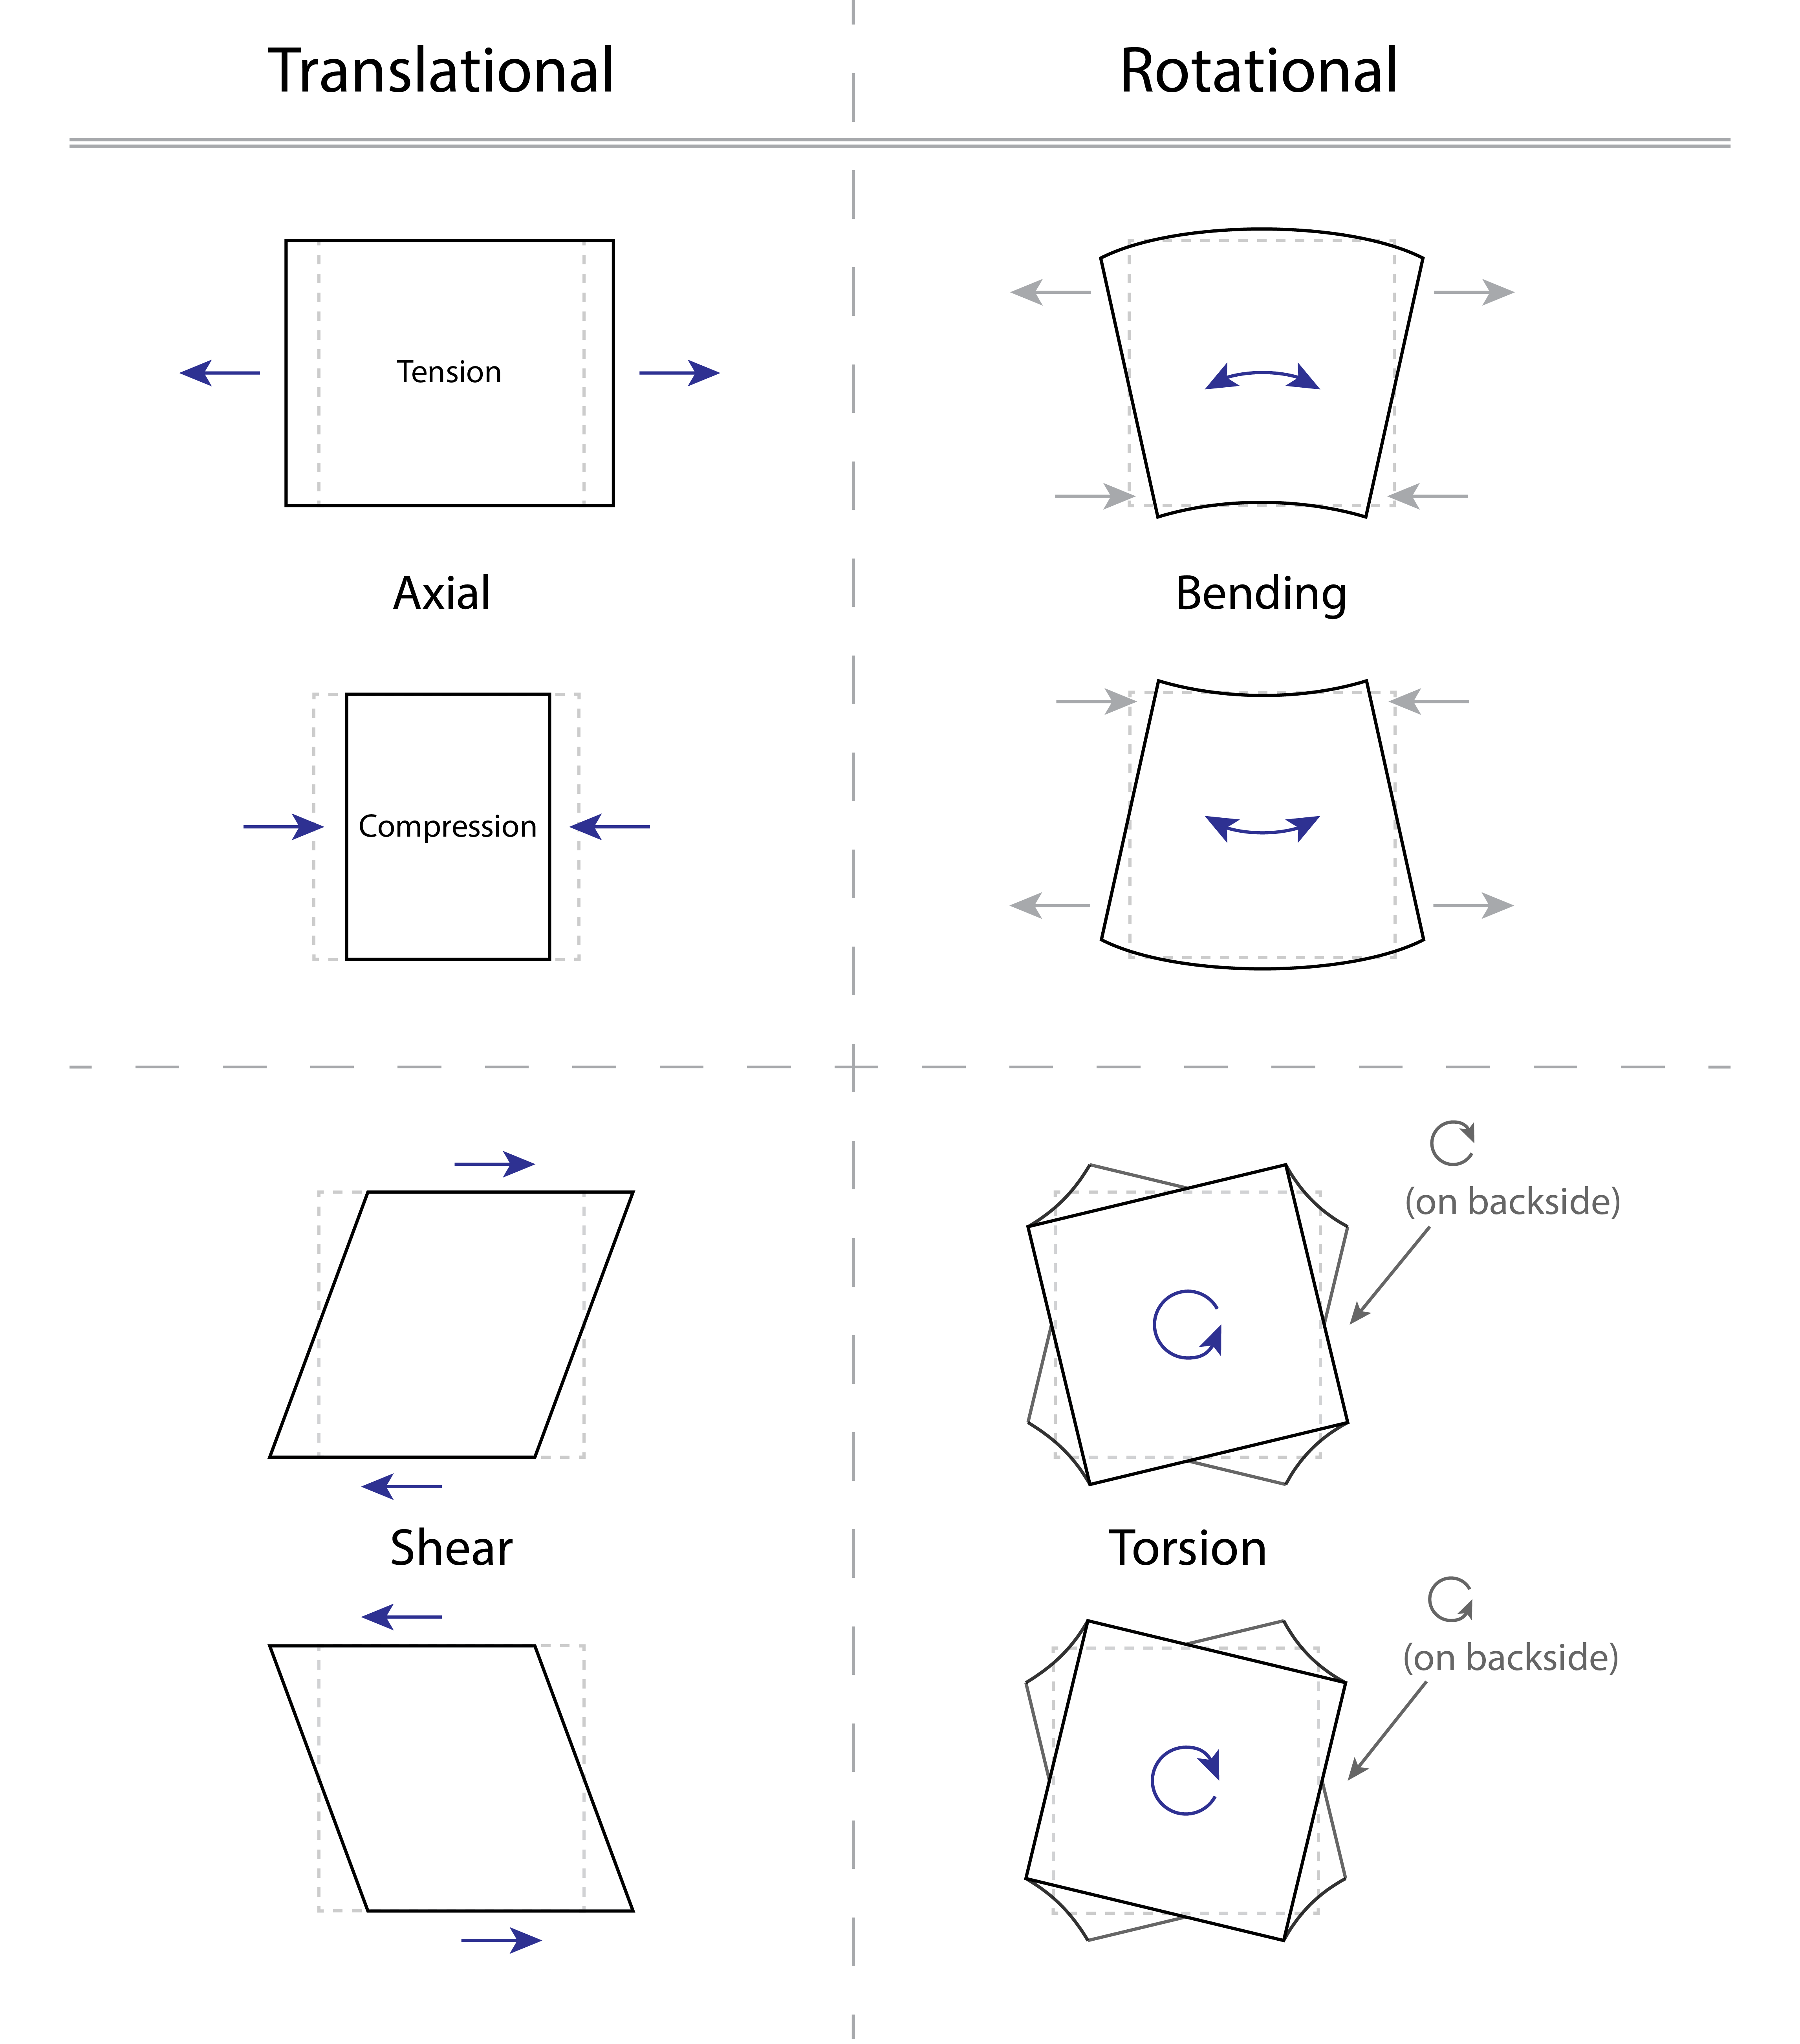
\includegraphics[width=\linewidth]{SolidMechanicsDOF.png}
  \caption{Deformations of a solid element under four types of applied forces.  In modeling assemblies of \textit{functions}, these characteristic deformations are referred to as "internal degrees of freedom".  Within an assembly of cells, longitudinal (compression and tension) and shear forces cause translational displacement and bending and torsional forces cause rotational displacement.}
  \label{fig:SolidMechanicsDOF}
\end{figure}

In solid mechanics, we can consider the global deformations of a solid as the summation of deformations of many smaller, discrete volumes, or \textit{finite elements}.  Forces acting on these finite elements fall into four categories: longitudinal (tension and compression), bending, shear, and torsion.  Each type of applied force causes a characteristic deformation of the finite element, illustrated in Figure \ref{fig:SolidMechanicsDOF}.  Applying multiple types of forces on a finite element will cause it to exhibit a combination of deformations.\\

In this model, simulation of an assembly happens at the granularity of identically-sized \textit{function}-level parts, which we'll call "cells".  When describing mechanical behavior of a particular cell type, we refer to its deformations as "internal degrees of freedom" (DOF).  For example, a 1-DOF bending cell will have large deformations in bending along one axis, but relatively small deformations in response to other types of applied forces.\\

\section{Function Types}

Cells at the function-level are defined not only by their mechanical properties, but also by their ability to transmit electronic signals from one face to another, and their active properties in response to a signal. The combinatorial space of mechanical, electronic, and actuated cell types is described in Figure \ref{fig:CombinatoricsOfFunctions}.  Section \ref{sec:electronicSim} describes the process of electronic simulation in more detail, the remainder of this chapter will focus on the passive and active mechanical simulation of function-level cells.
\\

\begin{figure}
  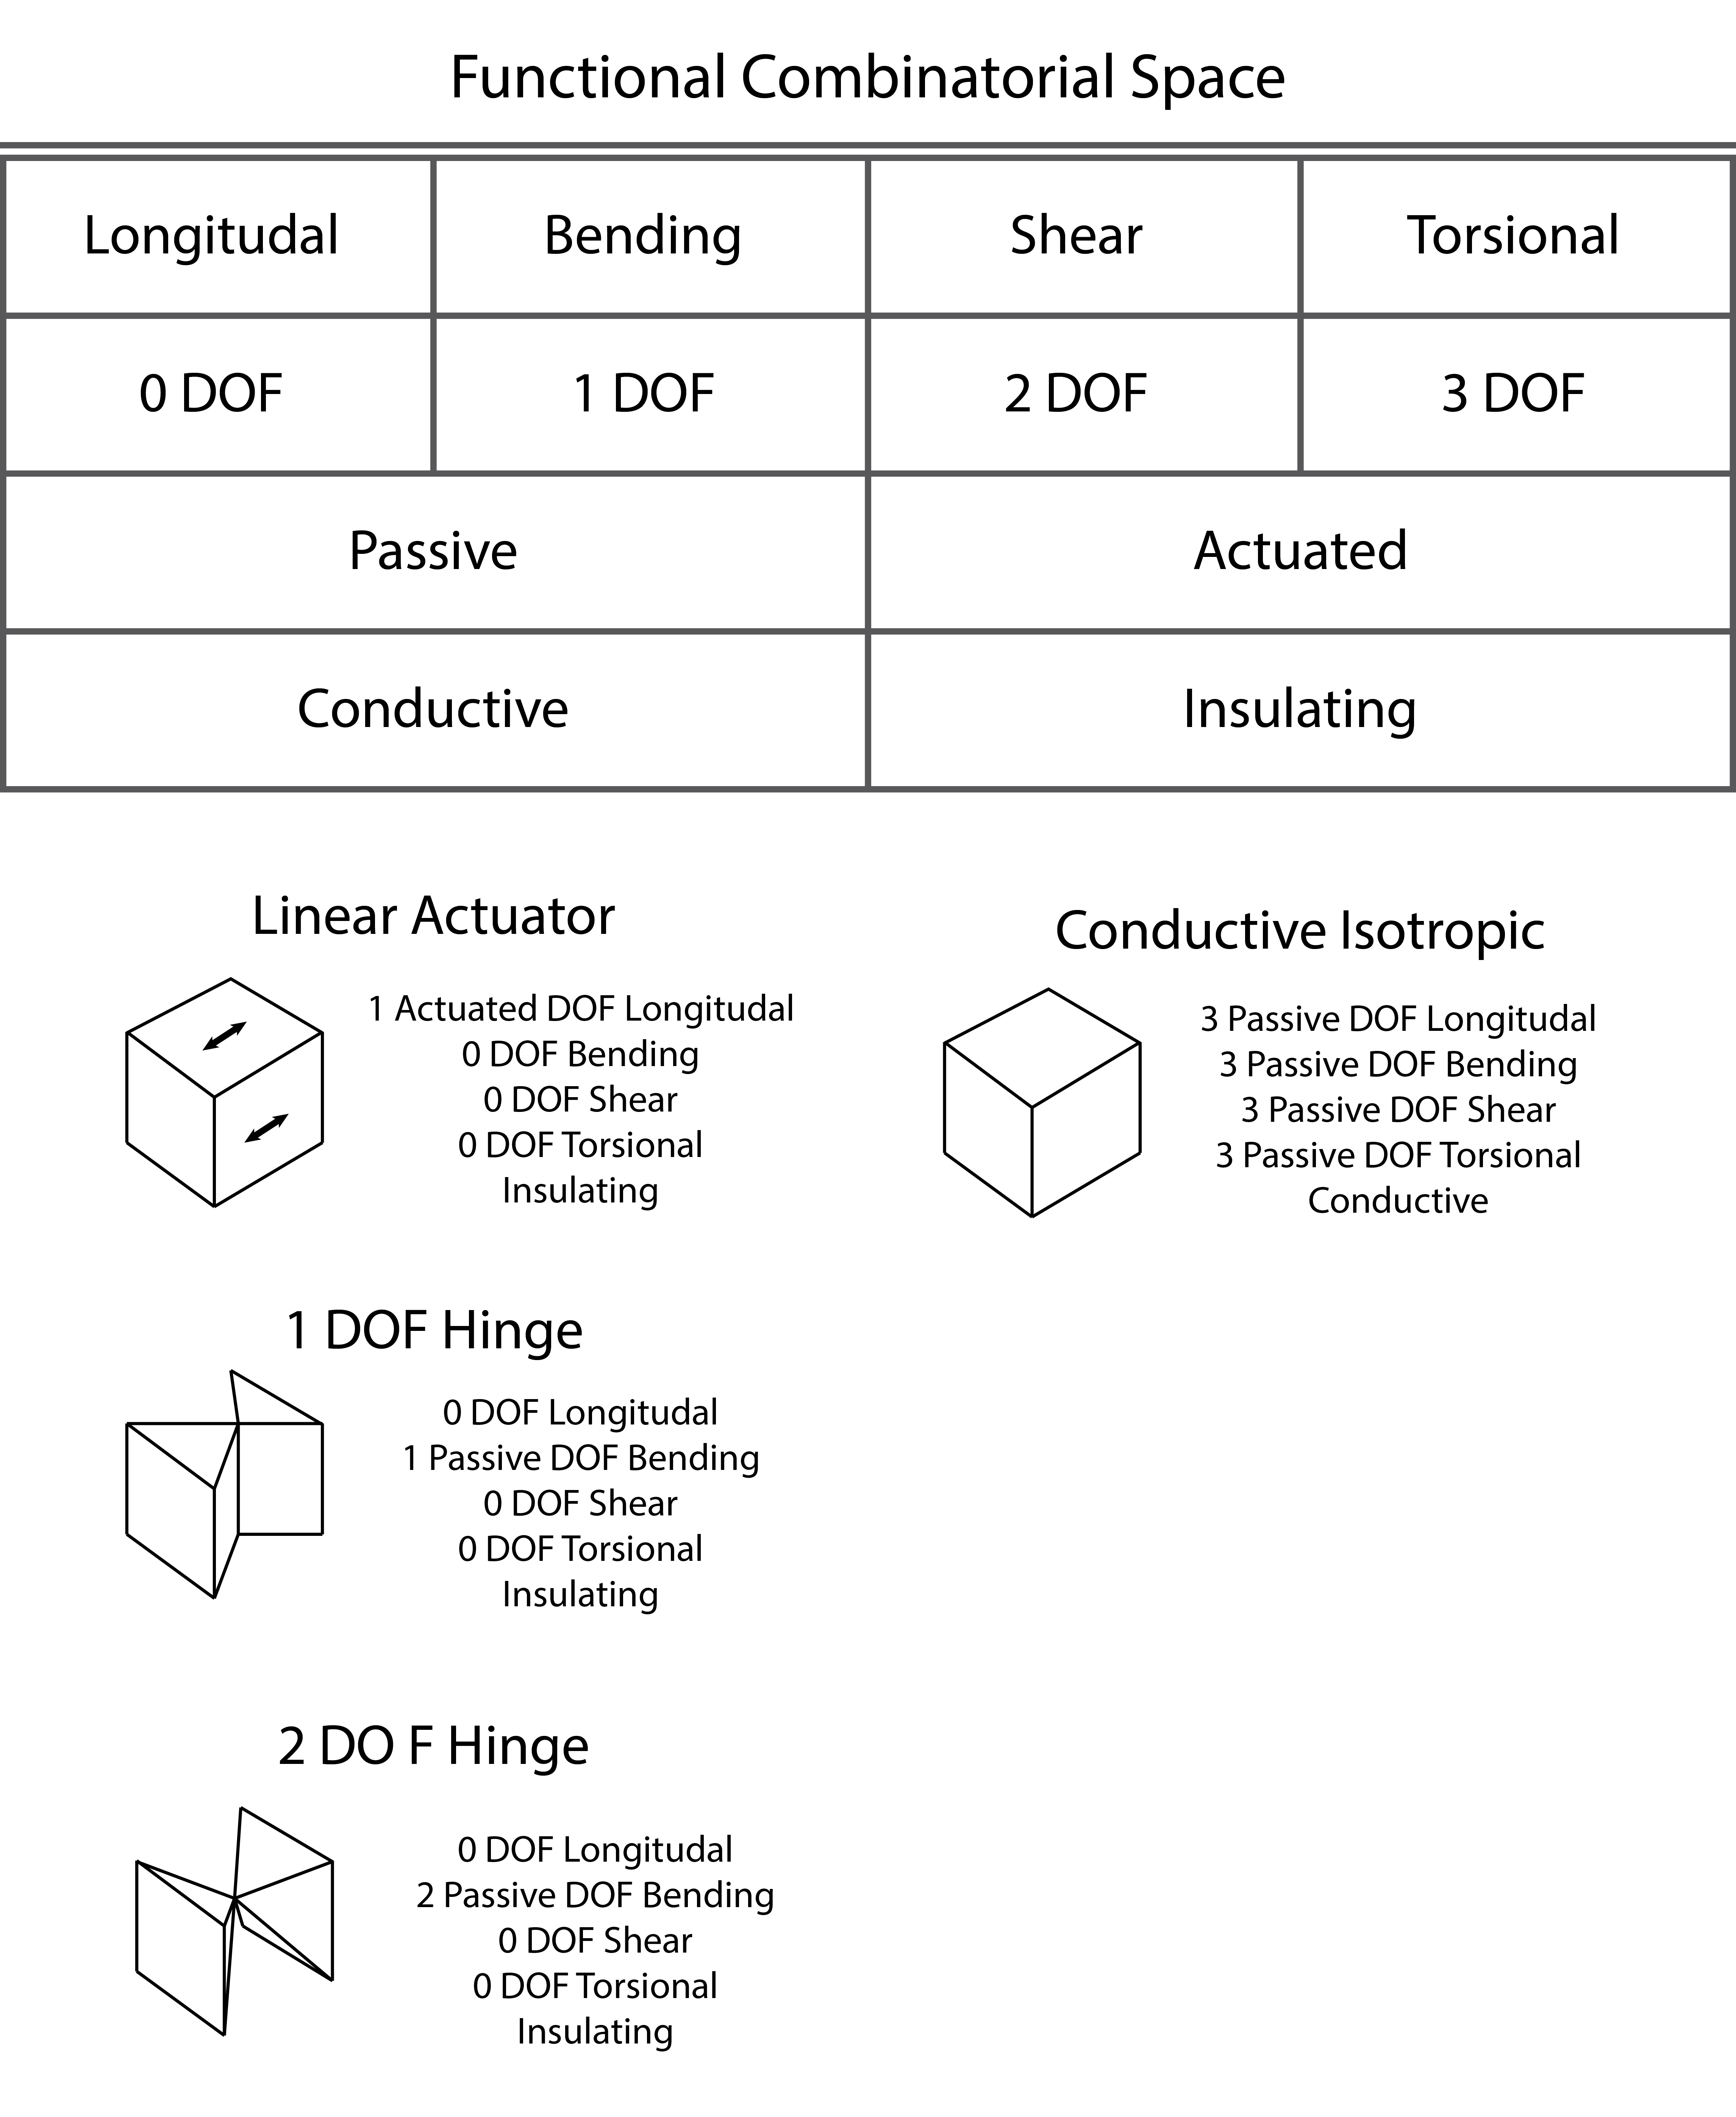
\includegraphics[width=\linewidth]{CombinatoricsOfFunctions.png}
  \caption{Combinatorial space of \textit{function} types with six examples explicitly described in terms of their electronic and mechanical properties.  Note - any individual degree of freedom within a cell falls on the spectrum described in Figure \ref{fig:BendingStiffnessContinuoum}.  A cell is described at a high level as having a particular degree of freedom if its corresponding stiffness in that dimension is sufficiently flexible to allow for significant deformation uder applled load.  There are no infinitely stiff or fully unconstrained degrees of freedom in this system.}
  \label{fig:CombinatoricsOfFunctions}
\end{figure}

A linear scale showing the range of physically achievable 1-DOF bending cell types compared with the range of theoretically possible types is shown in Figure \ref{fig:BendingStiffnessContinuoum}.  Due to manufacturing and material constraints, we do not envision \textit{function}-level cells that occupy the region near zero bending stiffness (e.g. a frictionless pin joint) or infinite bending stiffness (zero compliance material).

\begin{figure}
  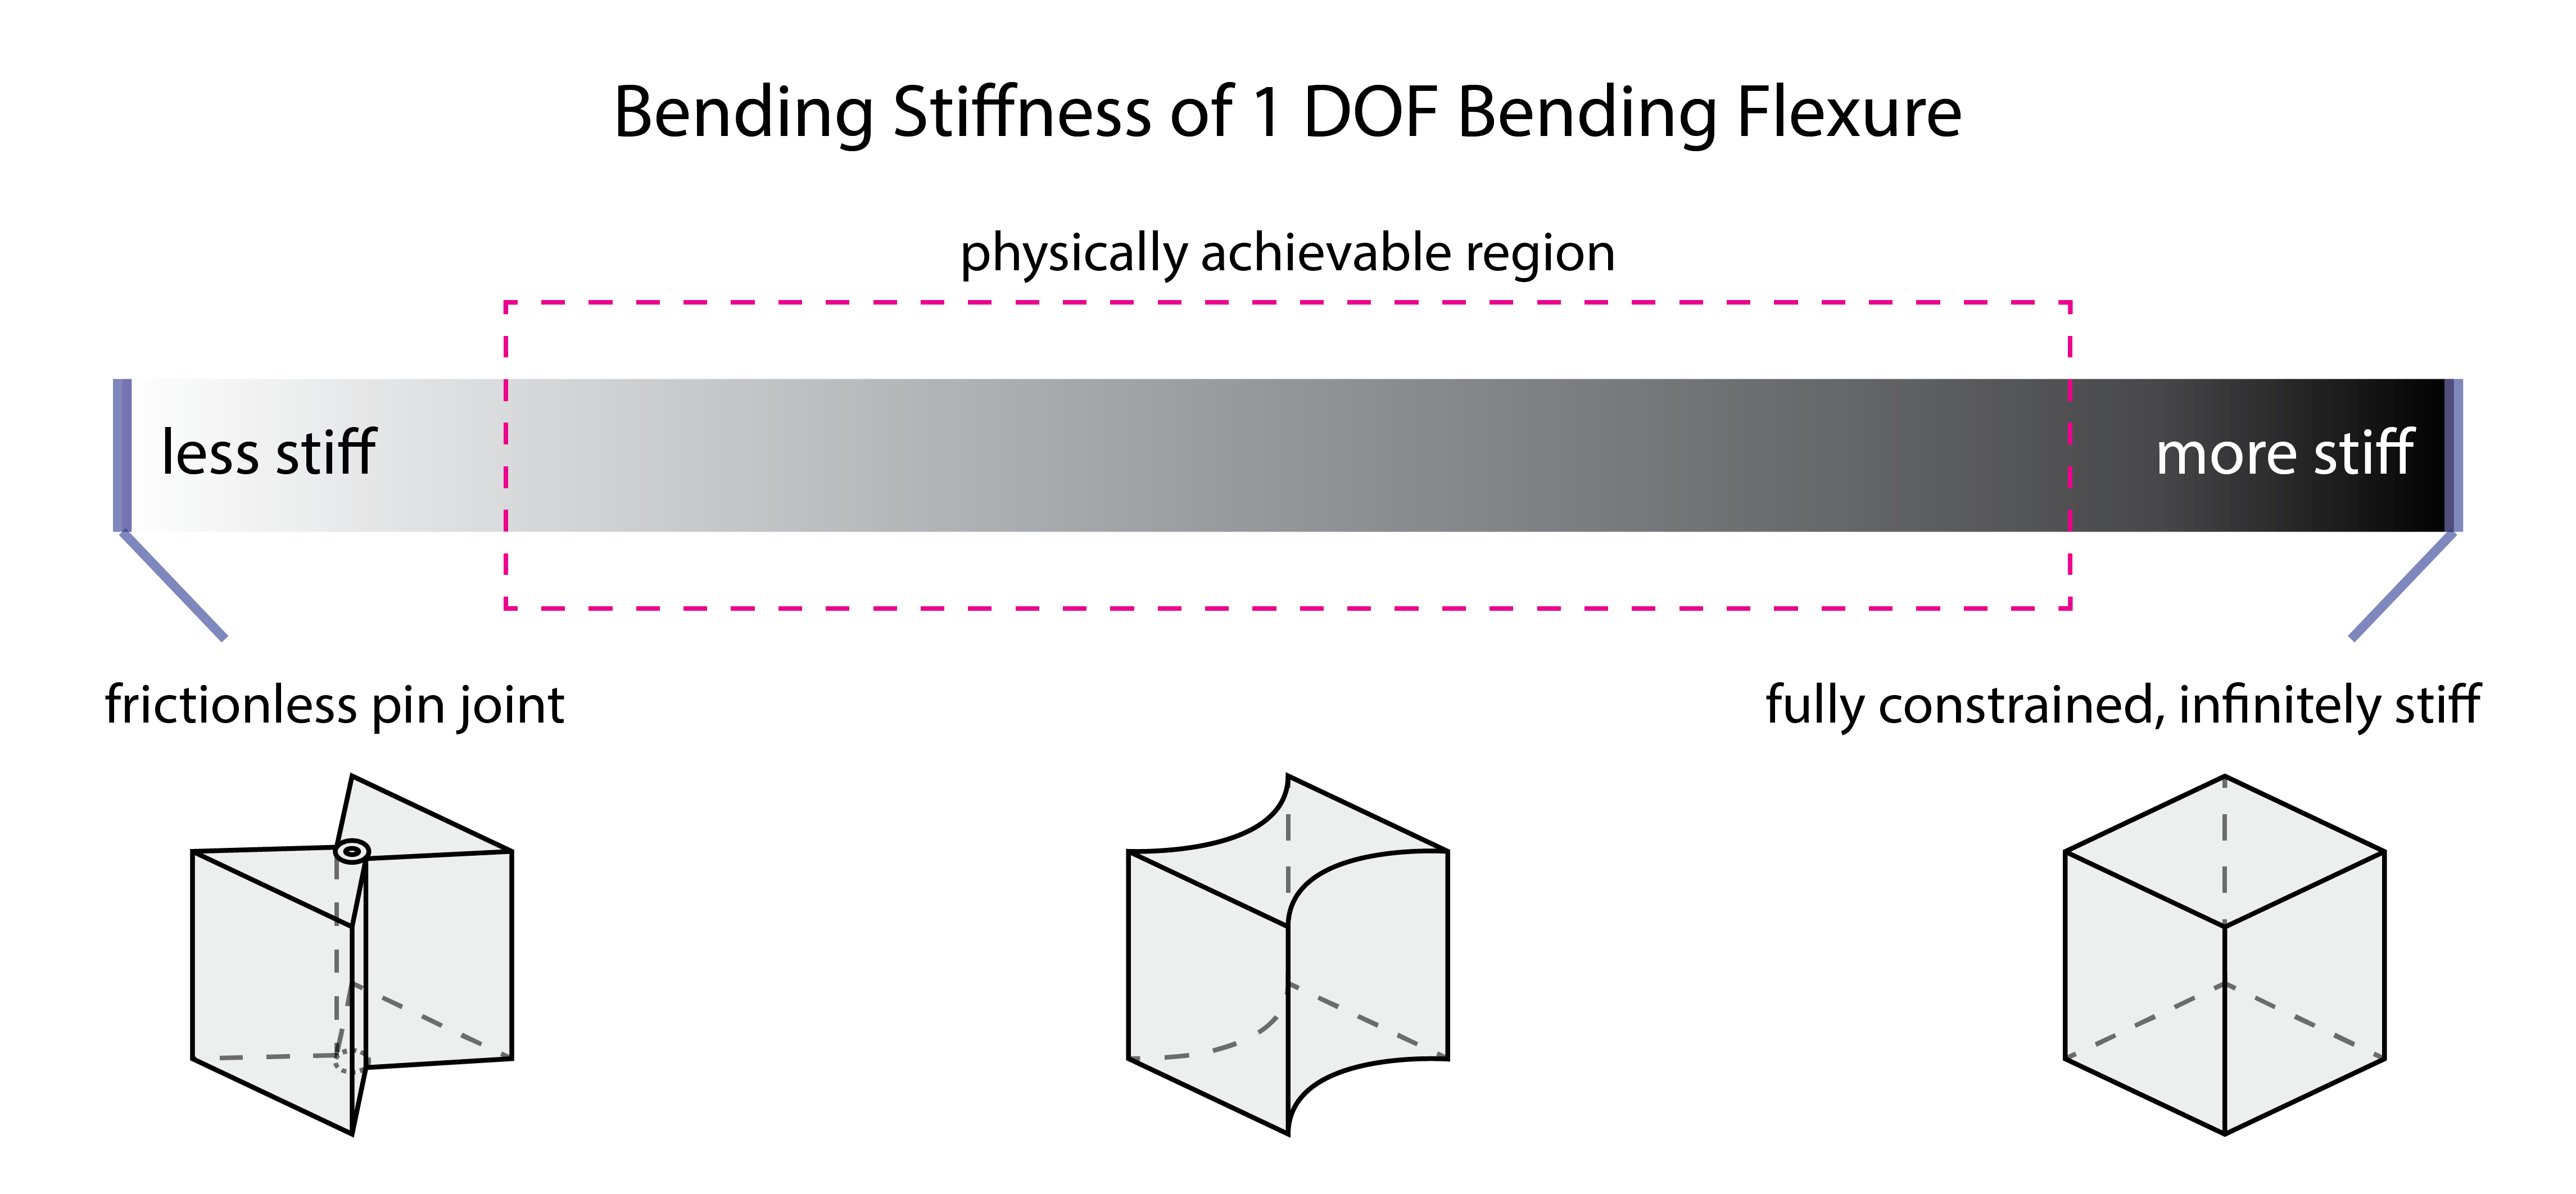
\includegraphics[width=\linewidth]{BendingStiffnessContinuoum.png}
  \caption{Continuum of bending stiffness in a 1 DOF hinge.}
  \label{fig:BendingStiffnessContinuoum}
\end{figure}

\section{Spring-Damper Characteristics}

The geometric stiffness of a structure relates the bulk properties of a material to its 3d geometry.  For example, an I-beam has a higher geometric bending stiffness than an equal length rectangular bar made from the same amount of the same material.  Unless otherwise noted, "stiffness" in this analysis refers to geometric stiffness.\\

Stiffness and damping are used to characterize the response of cell's internal degrees of freedom to applied external forces.  In three dimensions, each cell's passive mechanical properties are parameterized by 15 stiffness and damping constants:

\[ k  \left\{ \begin{array}{ccc}
k_{longitudinal_x}\\
k_{longitudinal_y}\\
k_{longitudinal_z}\\
\\
k_{shear_{xy}}\\
k_{shear_{xz}}\\
k_{shear_{yx}}\\
k_{shear_{yz}}\\
k_{shear_{zx}}\\
k_{shear_{zy}}\\
\\
k_{bending_x}\\
k_{bending_y}\\
k_{bending_z}\\
\\
k_{torsional_x}\\
k_{torsional_y}\\
k_{torsional_z}
 \end{array} \right\} 
 \qquad\qquad
 d  \left\{ \begin{array}{ccc}
d_{longitudal_x}\\
d_{longitudal_y}\\
d_{longitudal_z}\\
\\
d_{shear_{xy}}\\
d_{shear_{xz}}\\
d_{shear_{yx}}\\
d_{shear_{yz}}\\
d_{shear_{zx}}\\
d_{shear_{zy}}\\
\\
d_{bending_x}\\
d_{bending_y}\\
d_{bending_z}\\
\\
d_{torsional_x}\\
d_{torsional_y}\\
d_{torsional_z}
 \end{array} \right\}  \]
\\

$k_{shear}$ and $d_{shear}$ are broken out into six parameters of the form $shear_{nm}$ because the shear response depends both on the direction of shear displacement between two cells ($m$) and on the axis along which the cells are connected ($n$).  The $shear_{nm}$ notion used above is described graphically in in Figure \ref{fig:ShearDOFs}.\\

\begin{figure}
  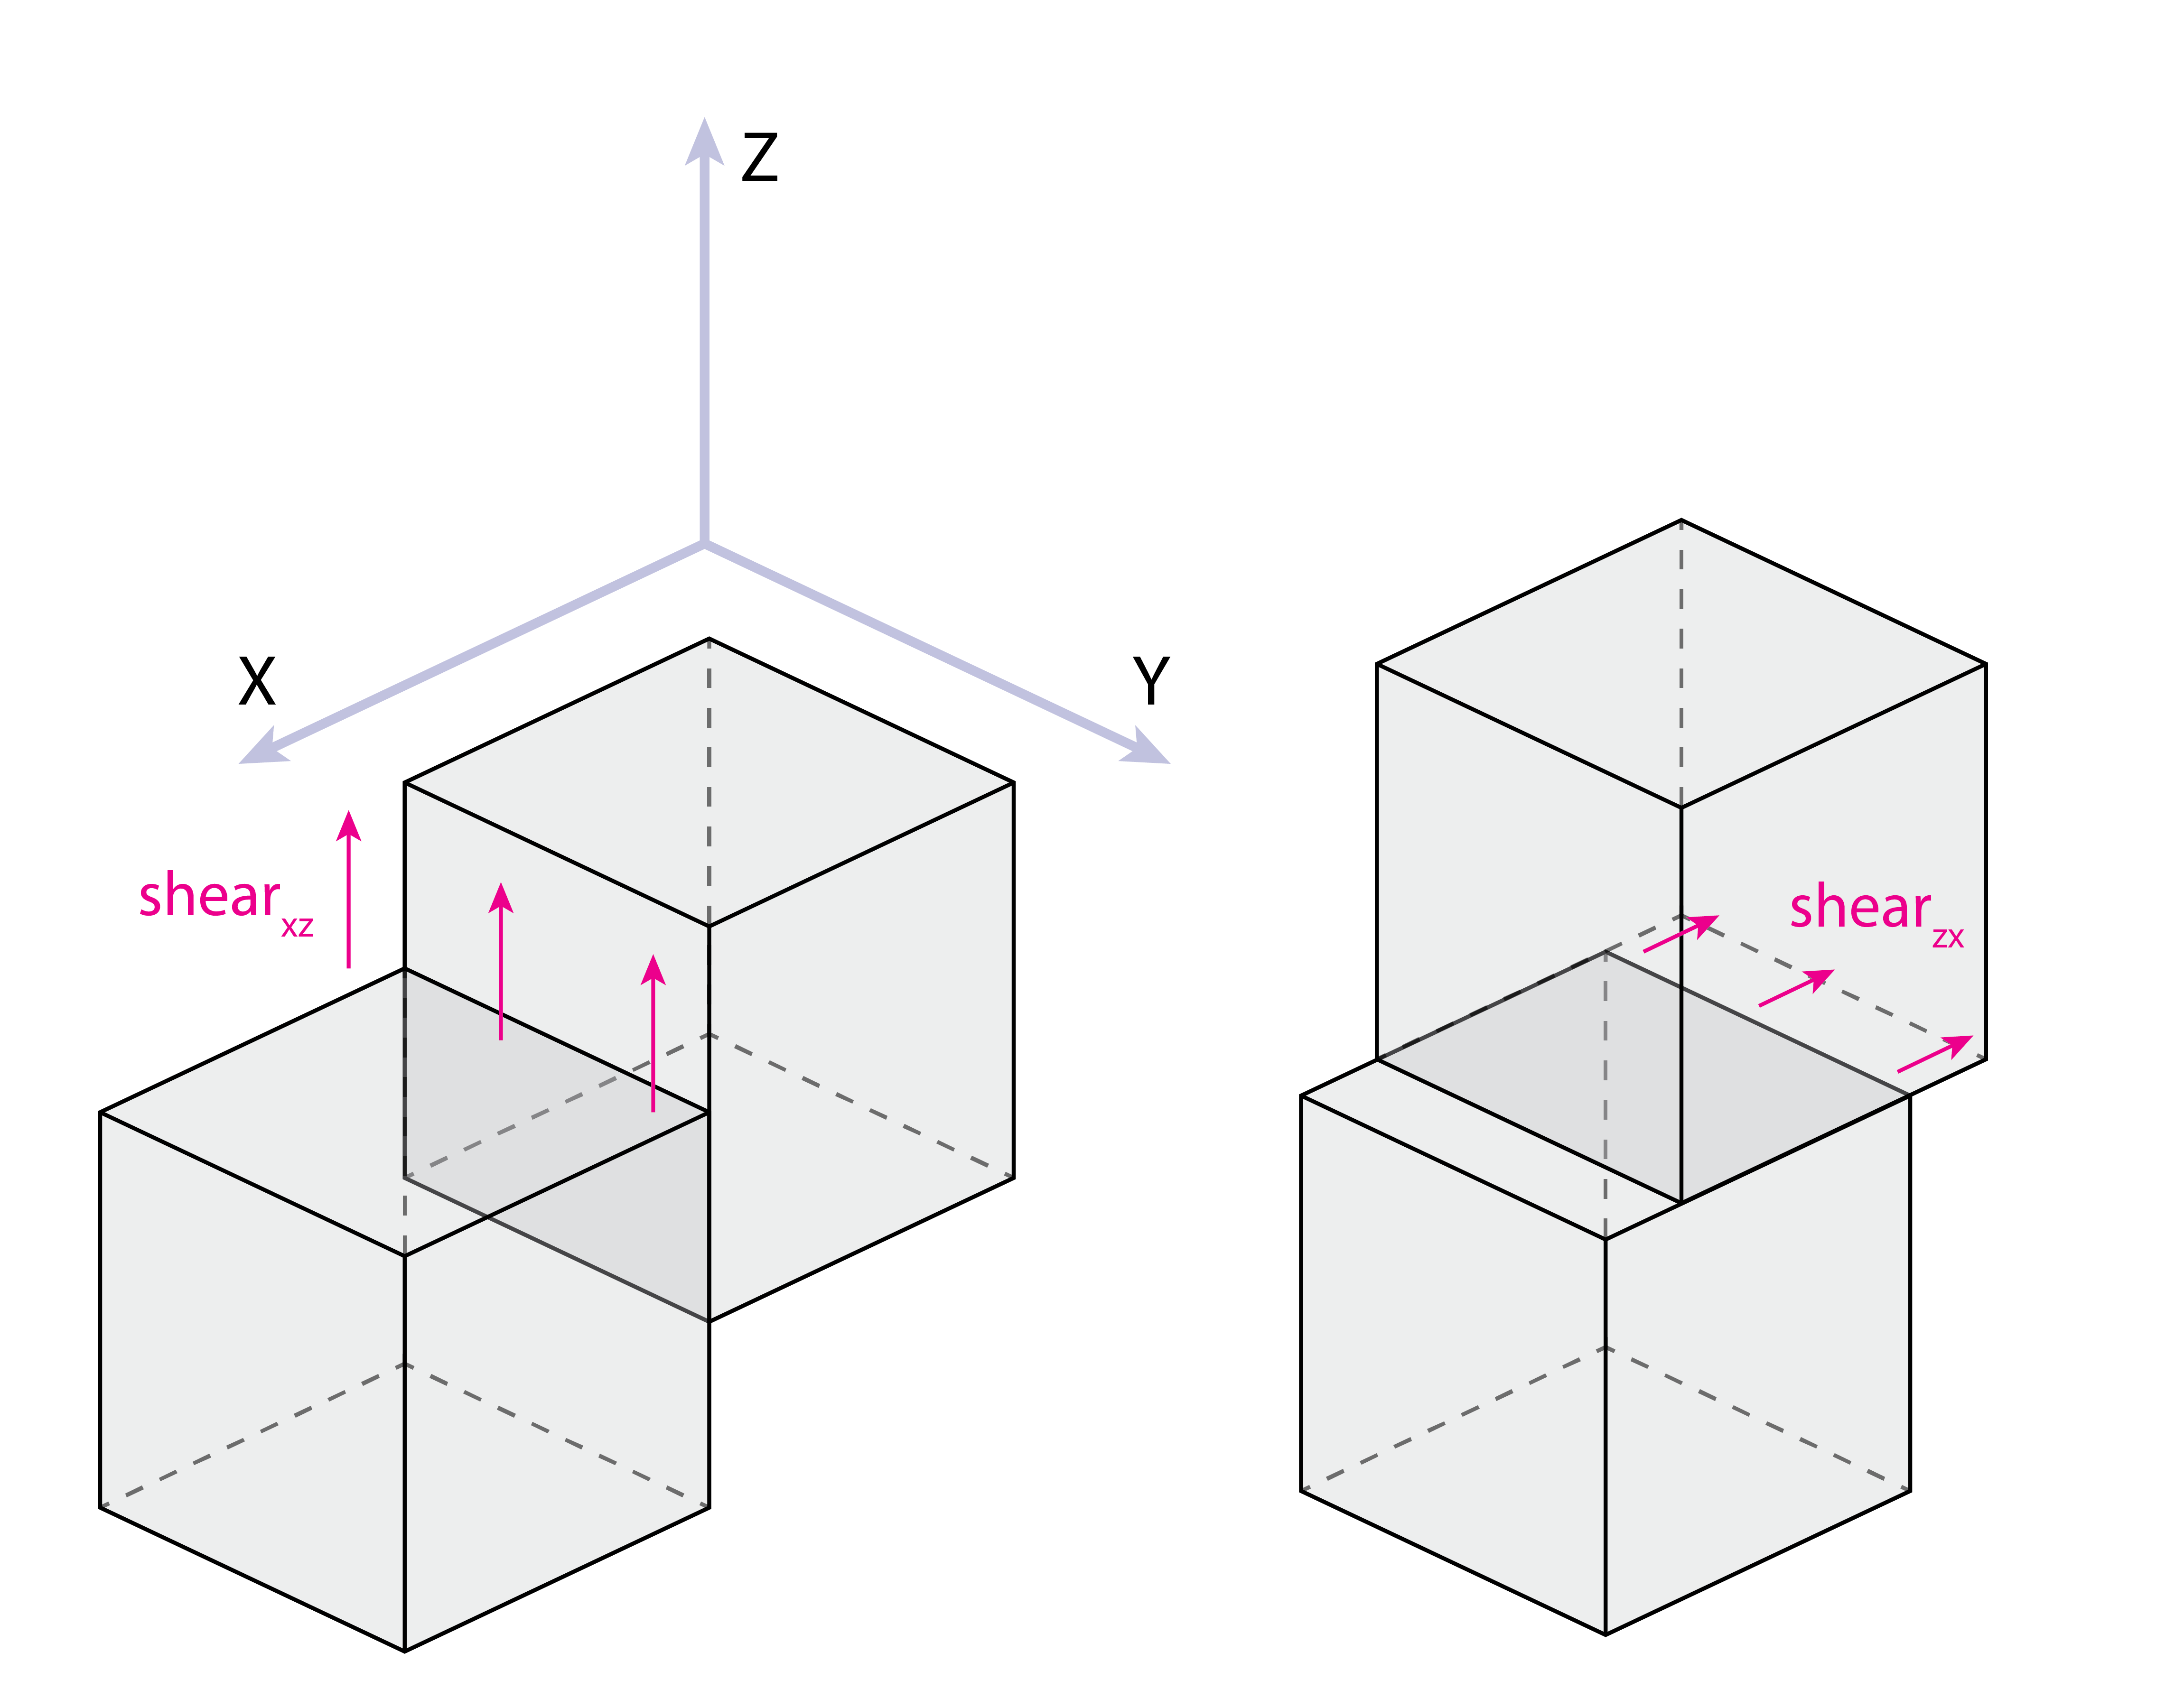
\includegraphics[width=\linewidth]{ShearDOFs.png}
  \caption{Illustration of shear subscript notation.  First subscript describes the direction of neighboring cell connection, second describes the direction of shear displacement.}
  \label{fig:ShearDOFs}
\end{figure}

The stiffness and damping constants of each cell type may be calculated from bulk properties of the constituent materials that make up the cell, or they may be measured empirically.  For example, an isotropic cell made from a bulk material with elastic modulus $E$ and shear modulus $G$ has stiffnesses defined by:

\[ k_{longitudinal} = \dfrac{aE}{l}\]
\[ k_{shear} = \dfrac{Ga}{l} ??\]
\[ k_{torsion} = \dfrac{GJ}{l}\]
\[ k_{bending} = \dfrac{aE}{l} ??\]
\\
where $a$ is the cross sectional area and $l$ is the length of the cell.\\

 In the case that the cells have different stiffness or damping constants, a composite stiffness or damping constant must be calculated in order to properly model the junction between the cells.  Composite stiffness can be calculated according to the following formula:
 \begin{equation} \label{eq:springseries}
 k_{composite} = \dfrac{2k_1k_2}{k_1+k_2}
 \end{equation}

similarly, composite damping is calculated by:
 \begin{equation} \label{eq:damperseries}
d_{composite} = \dfrac{2d_1d_2}{d_1+d_2}
 \end{equation}
 
 Equations \ref{eq:springseries} and \ref{eq:damperseries} are equivalent to the formulas for two springs or two dampers of half length in series.  This is demonstrated graphically in Figure \ref{fig:SeriesCoupling}.  Notice, for example, in the case of $k1=k2$, Equation \ref{eq:springseries} reduces to $ k_{composite} = k1 = k2$.\\
 
 \begin{figure}
  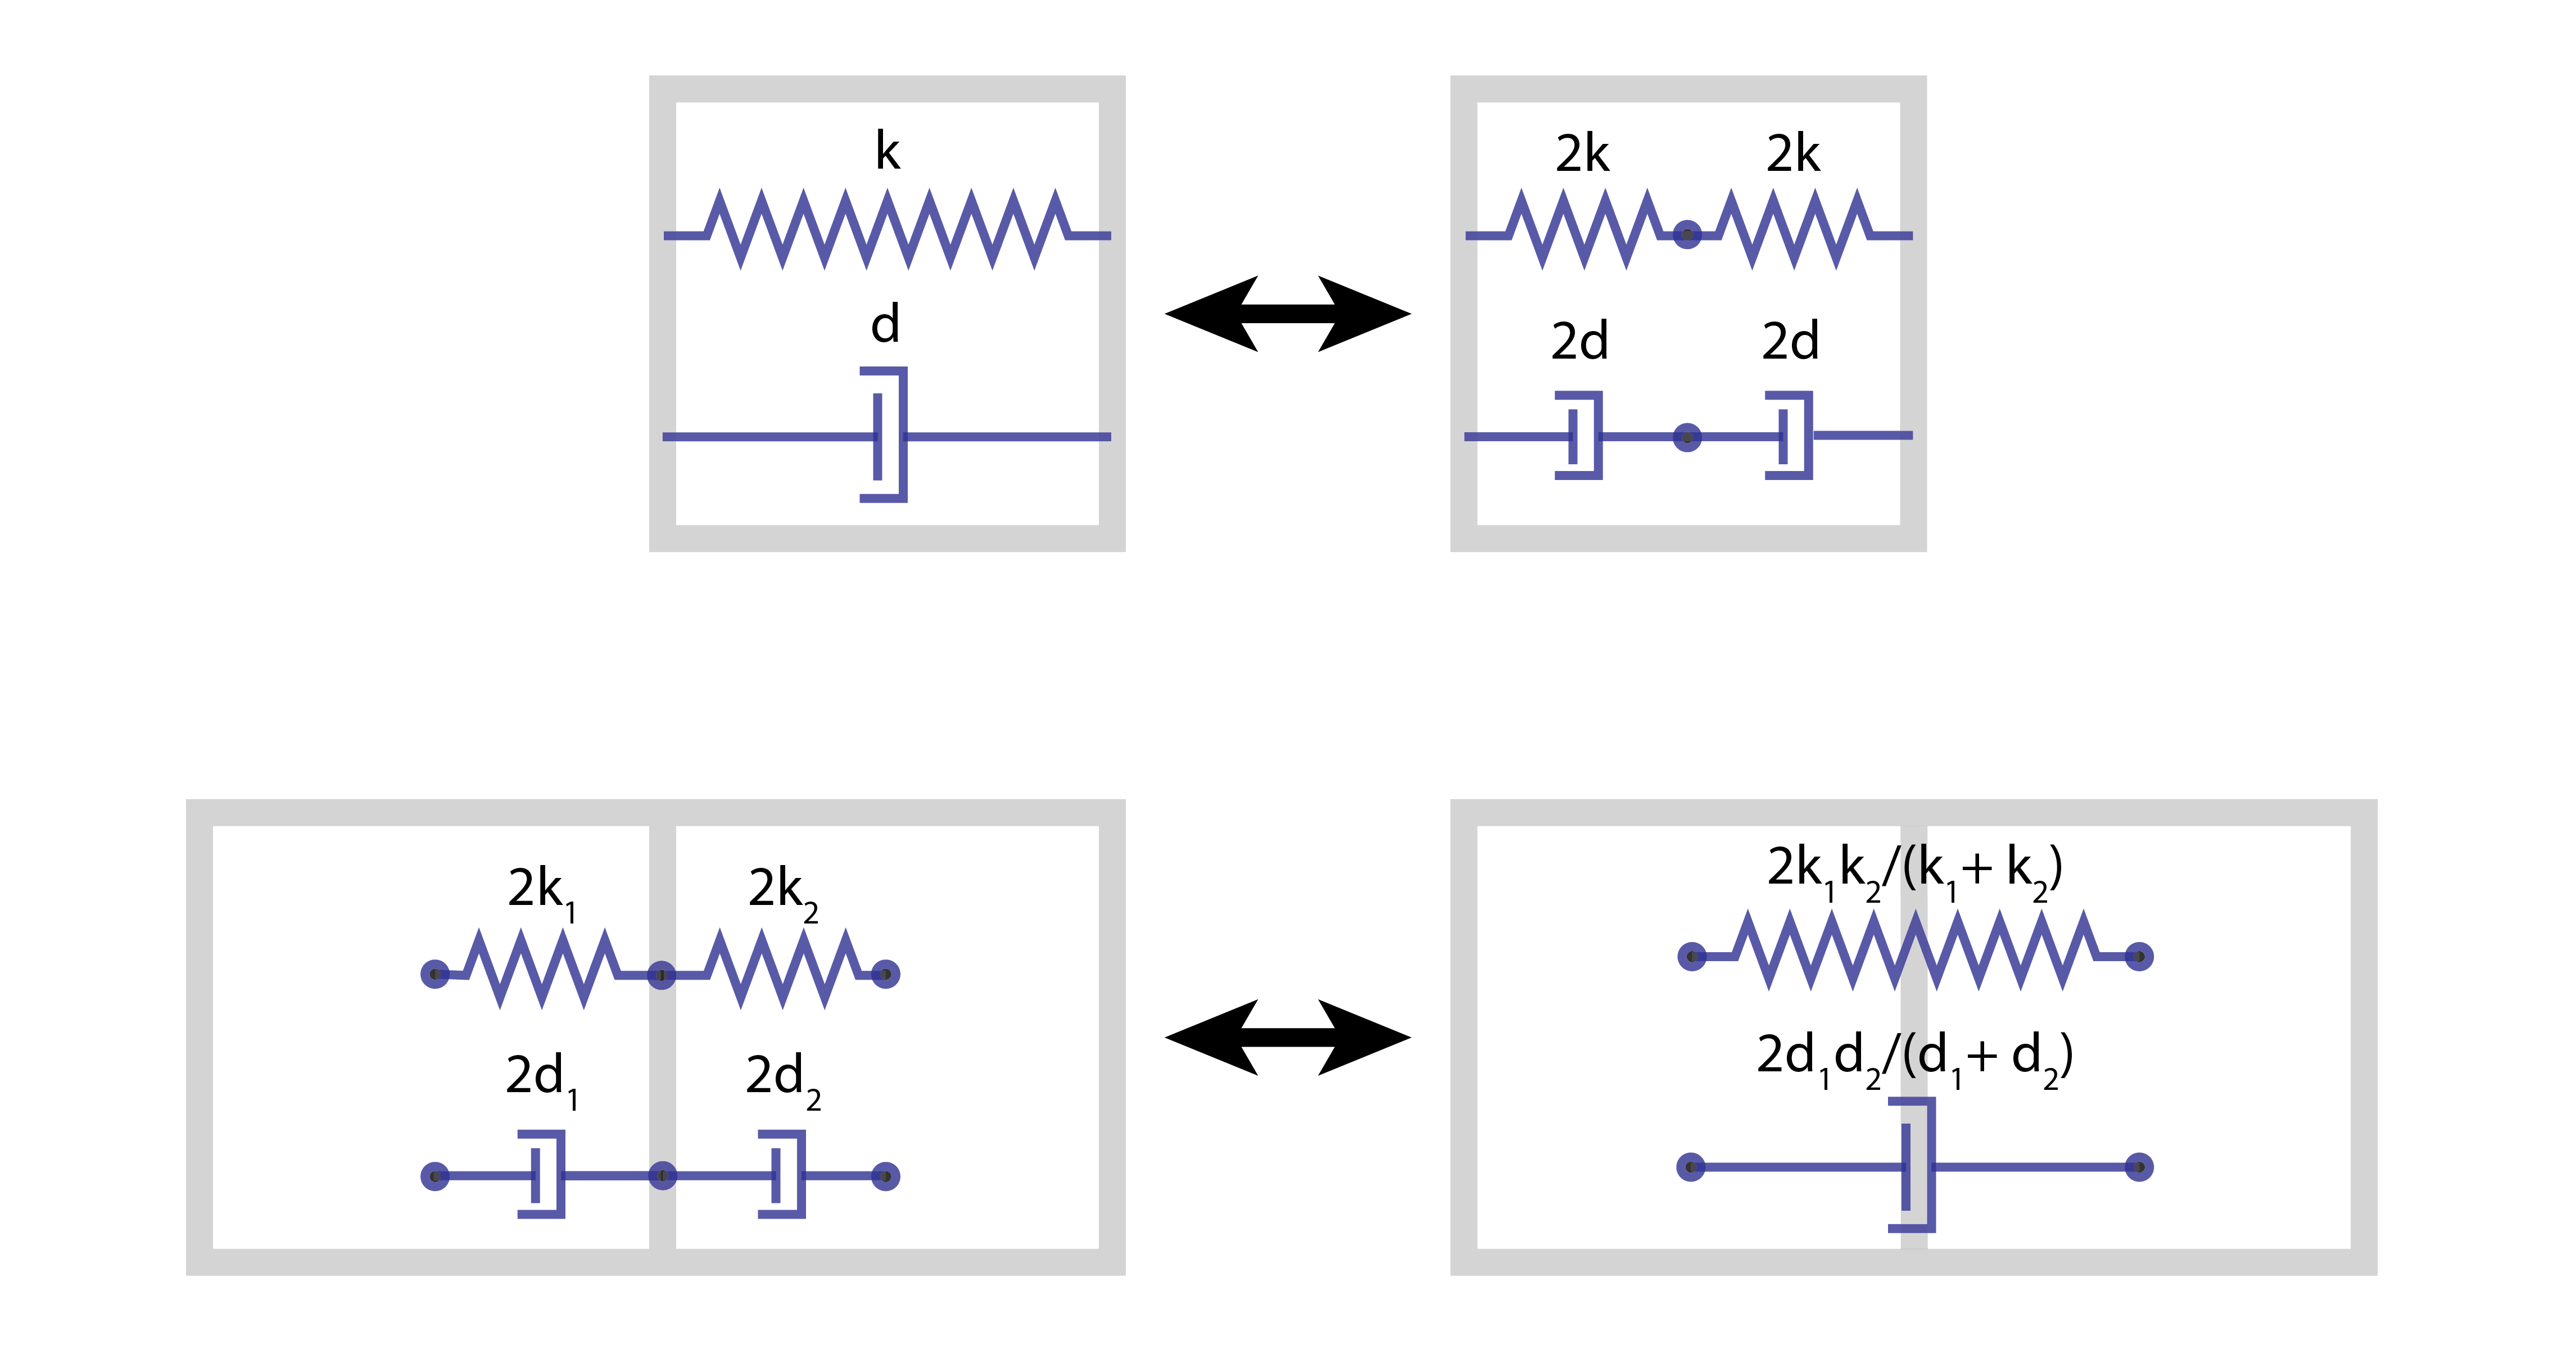
\includegraphics[width=\linewidth]{SeriesCoupling.png}
  \caption{Calculation of composite stiffness and damping of two cells with different k and d constants.}
  \label{fig:SeriesCoupling}
\end{figure}


\section{Translational Forces}

\begin{figure}
  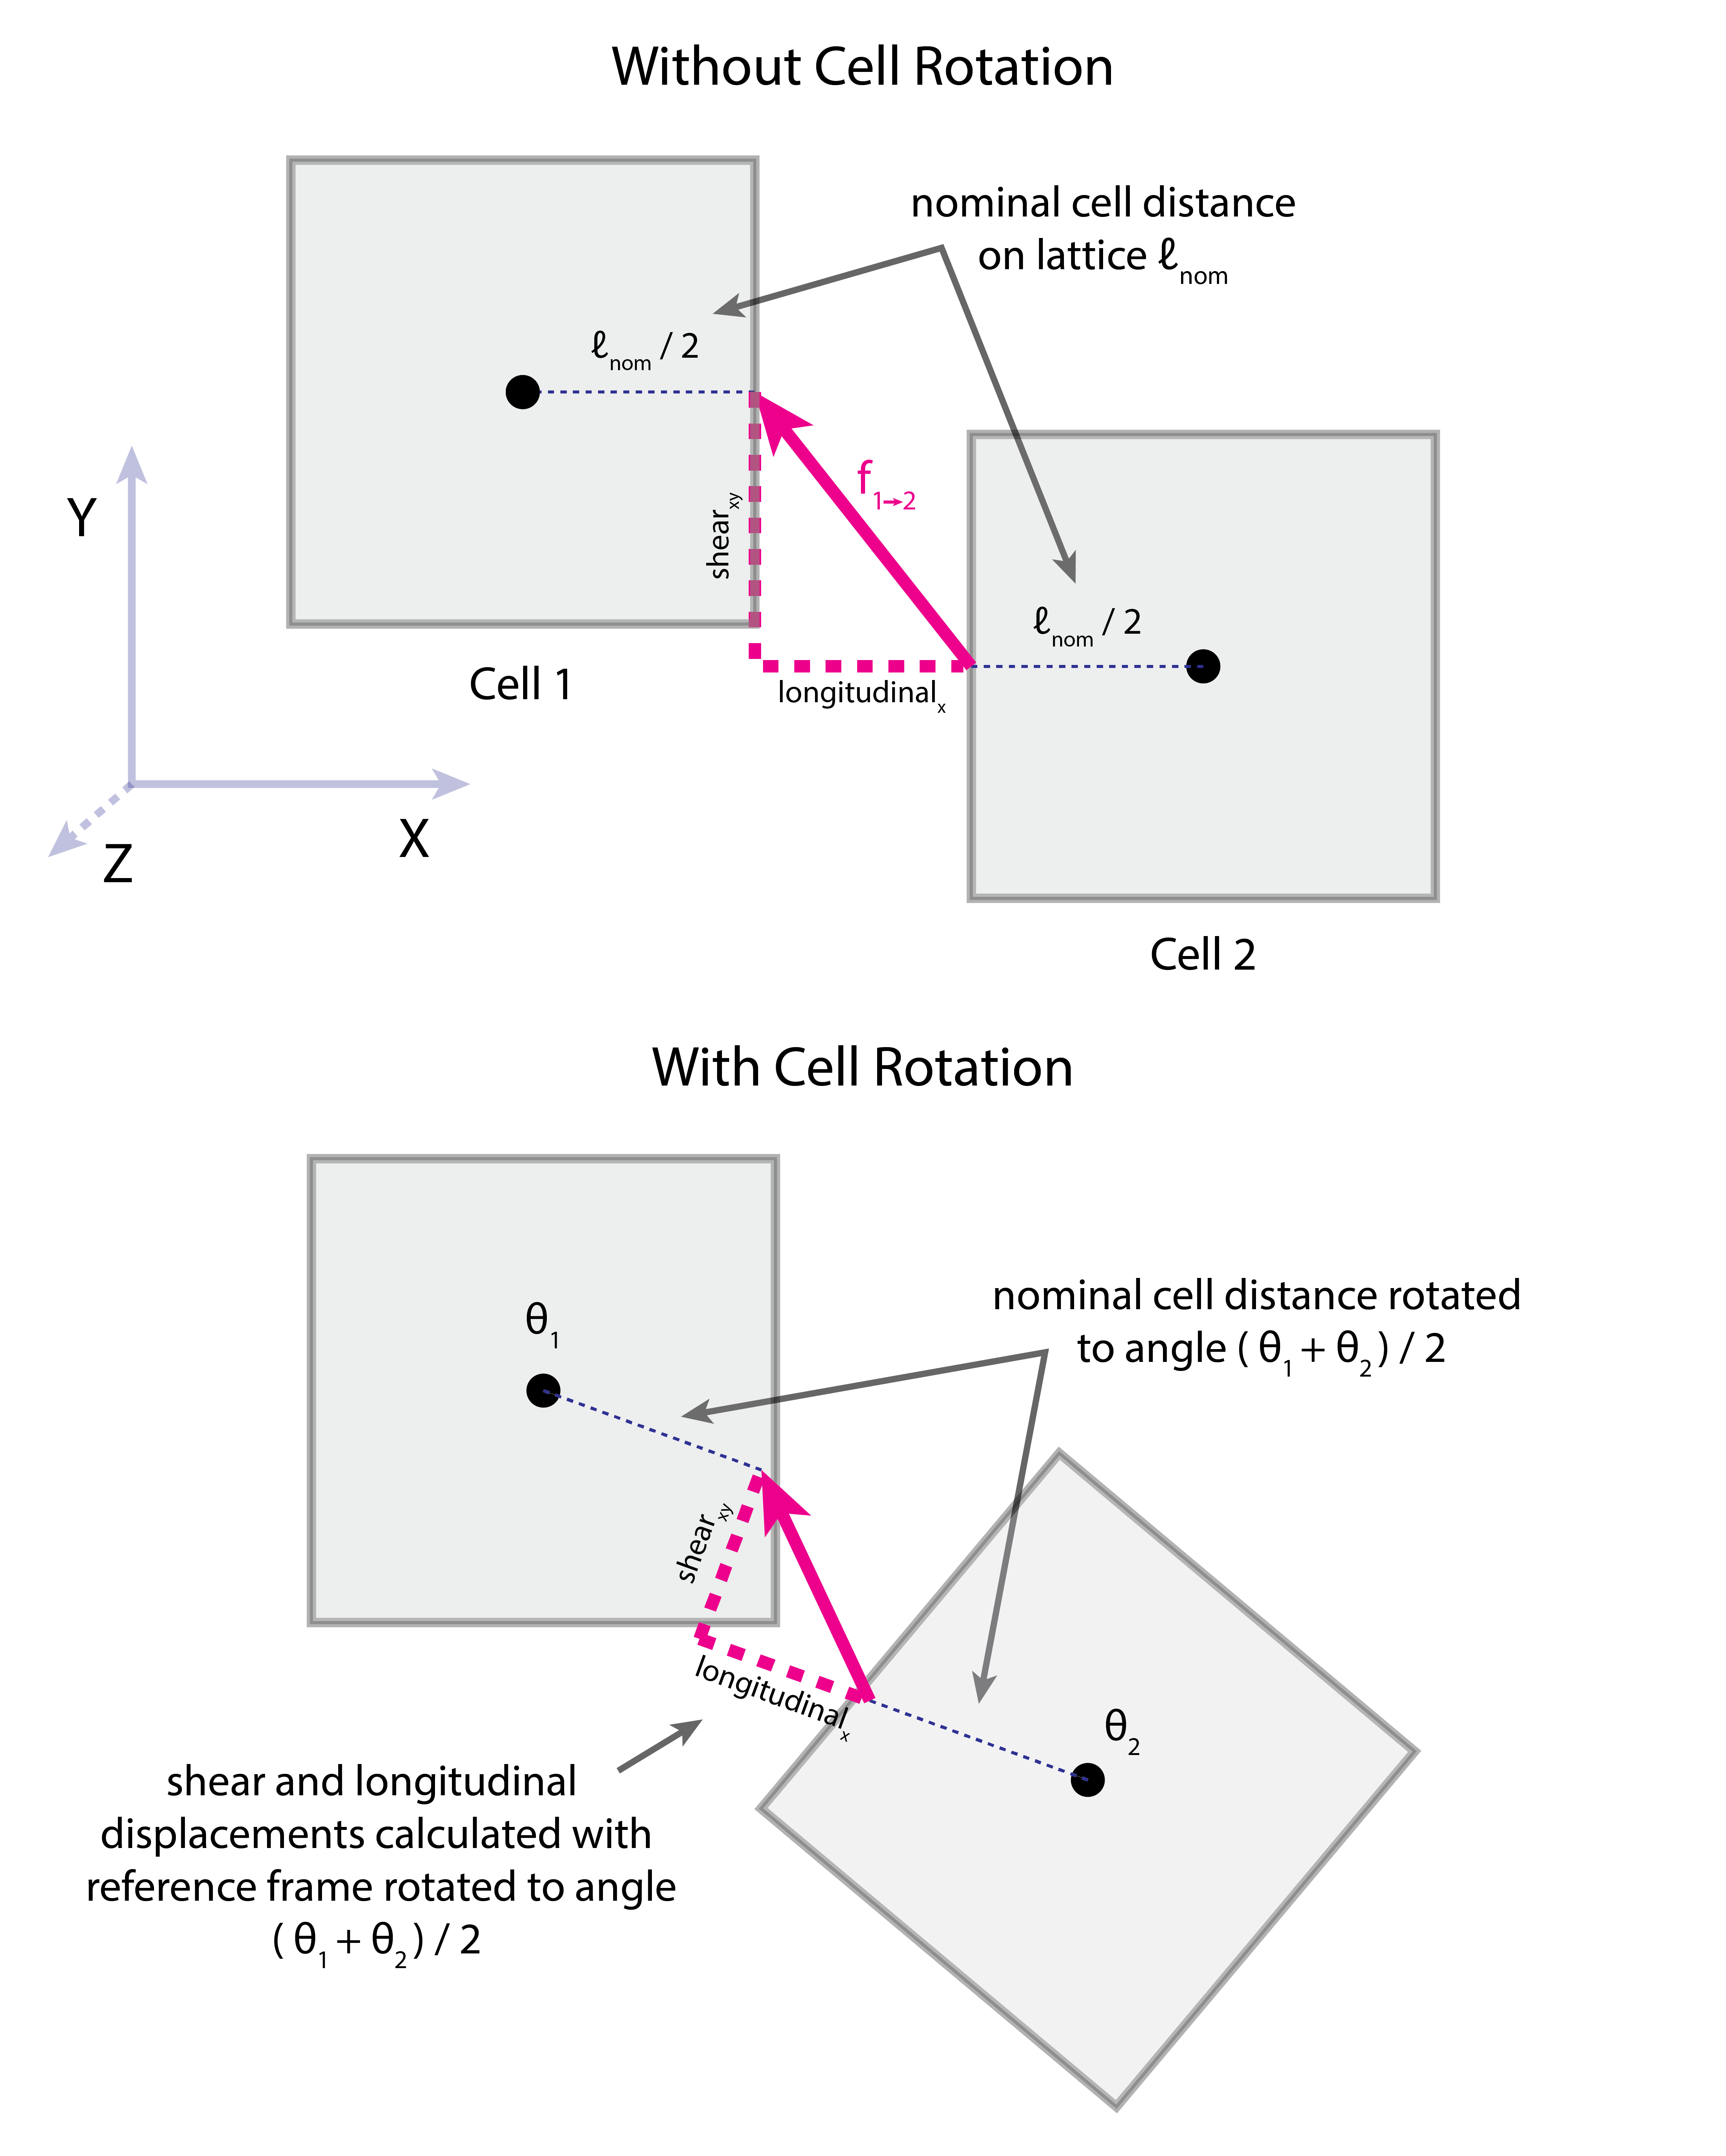
\includegraphics[width=\linewidth]{translationalSim.png}
  \caption{translationalSim.}
  \label{fig:translationalSim}
\end{figure}

In the simplest case without rotation, the force $\vec{f}_{1 \rightarrow 2}$ applied to cell 2 by cell 1 is given by:
\begin{equation} \label{eq:translationalForce}
\vec{f}_{1\rightarrow2} = \vec{k} \circ (\vec{p}_1 - \vec{p}_2) + \vec{d} \circ (\vec{v}_1 - \vec{v}_2)
\end{equation}

where $\vec{p}_1$ and $\vec{p}_2$ are the displacements of cell 1 and cell 2 from their nominal position in the lattice, $\vec{v}_1$ and $\vec{v}_2$ are the cells' translational velocities, $\circ$ is multiplication of two vectors by element, and $\vec{k}$ and $\vec{d}$ are 3D vectors containing the appropriate composite stiffness and damping constants for the interaction between the cells.  For example, given the scenario illustrated in Figure \ref{fig:translationalSim}, where two cells are connected along the x axis, a longitudinal constant should be used for displacements along x and shear constants should be used for displacements along y and z:
\[ \vec{k} =  \left[ \begin{array}{ccc}
k_{longitudinal_x}\\
k_{shear_{xy}}\\
k_{shear_{xz}}
 \end{array} \right]  
  \qquad\qquad
  \vec{d} =  \left[ \begin{array}{ccc}
d_{longitudinal_x}\\
d_{shear_{xy}}\\
d_{shear_{xz}}
 \end{array} \right] \] 
 
If we wish to consider the orientations of the cells, denoted by the unit quaternions $q1$ and $q2$, we will need to adjust equation \ref{eq:translationalForce}. \\
  
  We can rotate a vector $\vec{v}$ in 3-space by a quaternion $q$ in 4-space:
    \[ \vec{v}_{rotated} = q*\vec{v}*q^* \]
  
  by treating $\vec{v}$ as a 4-space vector $[x, y, z, w]$ with $w=0$.  The operator $*$ denotes the Hamilton product:
  \[ a*b =  \left[ \begin{array}{ccc}
a_wb_x + a_xb_w + a_yb_z - a_zb_y\\
a_wb_y - a_xb_z + a_yb_w + a_zb_x\\
a_wb_z + a_xb_y - a_yb_x + a_zb_w\\
a_wb_w - a_xb_x - a_yb_y - a_zb_z
 \end{array} \right] \] 
 
   and $q^*$ denotes the conjugate of $q$:
    \[ q^{*} =  \left[ \begin{array}{ccc}
-q_x\\
-q_y\\
-q_z\\
q_w
 \end{array} \right] \] 
 
By performing a spherical linear interpolation (slerp) halfway between $q1$ and $q2$, we can calculate the average orientation of the two cells as a unit quaternion:
  \[ q_{avg} = slerp(q_{1}, q_{2}; 0.5) \]
  
Using $q_{avg}$, we can rotate the stiffness and damping vectors from Equation \ref{eq:translationalForce} into this average reference frame, and substitute the rotated vectors back into equation \ref{eq:translationalForce}:

 \[ \vec{k}_{rot} = (q_{avg}*\vec{k}*q_{avg}^*)\]
  \[ \vec{d}_{rot} = (q_{avg}*\vec{d}*q_{avg}^*)\]
  \begin{equation} \label{eq:translationalForceRotStep}
 \vec{f}_{1\rightarrow2} = \vec{k}_{rot} \circ (\vec{p}_1 - \vec{p}_2) + \vec{d}_{rot} \circ (\vec{v}_1 - \vec{v}_2)
 \end{equation}
 
Finally, we need to make an adjustment to the nominal differential position between the cells, indicated in Figure \ref{fig:translationalSim}.  The form above assumes the nominal distance between the centers of the cells is the unrotated distance from cells 2 to cell 1 in their initial lattice configuration, $\vec{l}_{nom21}$:
 \[\vec{l}_{nom21} = \vec{p}_{abs2}-\vec{p}_{abs1}\]
 
 where $\vec{p}_{abs}$ is the absolute position of a cell in the world reference frame.
 Rotating $\vec{l}_{nom}$ into the average rotational reference frame of the two cells gives
 \[\vec{l}_{rot21} = q_{avg}*\vec{l}_{nom21}*q_{avg}^*\]
 
introducing this correction to Equation \ref{eq:translationalForceRotStep} gives the final form:
 \begin{equation} \label{eq:translationalForceRot}
  \vec{f}_{1\rightarrow2} = \vec{k}_{rot} \circ (\vec{p}_1 - \vec{p}_2 + \vec{l}_{nom21}-\vec{l}_{rot21}) + \vec{d}_{rot} \circ (\vec{v}_1 - \vec{v}_2)
  \end{equation}

The force $\vec{f}_{2\rightarrow1}$ exerted on cell 2 by cell 1 is equal in magnitude to $\vec{f}_{1\rightarrow2}$ and opposite in direction:
\[  \vec{f}_{2\rightarrow1} = -\vec{f}_{1\rightarrow2} = \vec{k}_{rot} \circ (\vec{p}_1 - \vec{p}_2 + \vec{l}_{nom12}-\vec{l}_{rot12}) + \vec{d}_{rot} \circ (\vec{v}_1 - \vec{v}_2) \]

Only $\vec{f_{1\rightarrow2}}$ is indicated with a solid pink arrow in Figure \ref{fig:translationalSim}.\\

Dividing by the mass, we can calculate the acceleration of cells 1 and 2 due to interactions between them:

 \[ \vec{a}_{1\rightarrow2} = \dfrac{\vec{f}_{1\rightarrow2}}{m_2} 
  \qquad\qquad
   \vec{a}_{2\rightarrow1} = \dfrac{\vec{f}_{2\rightarrow1}}{m_1} 
  \]

\section{Rotational Forces}

So far, this model uses shear and longitudinal stiffness and damping constants to compute the translational interactions between neighboring cells in 3D.  In order to incorporate bending and torsional forces, we must develop a method of for cells to apply torques to one another.  These torques result in rotational motion of a cell about its center of mass.\\

\begin{figure}
  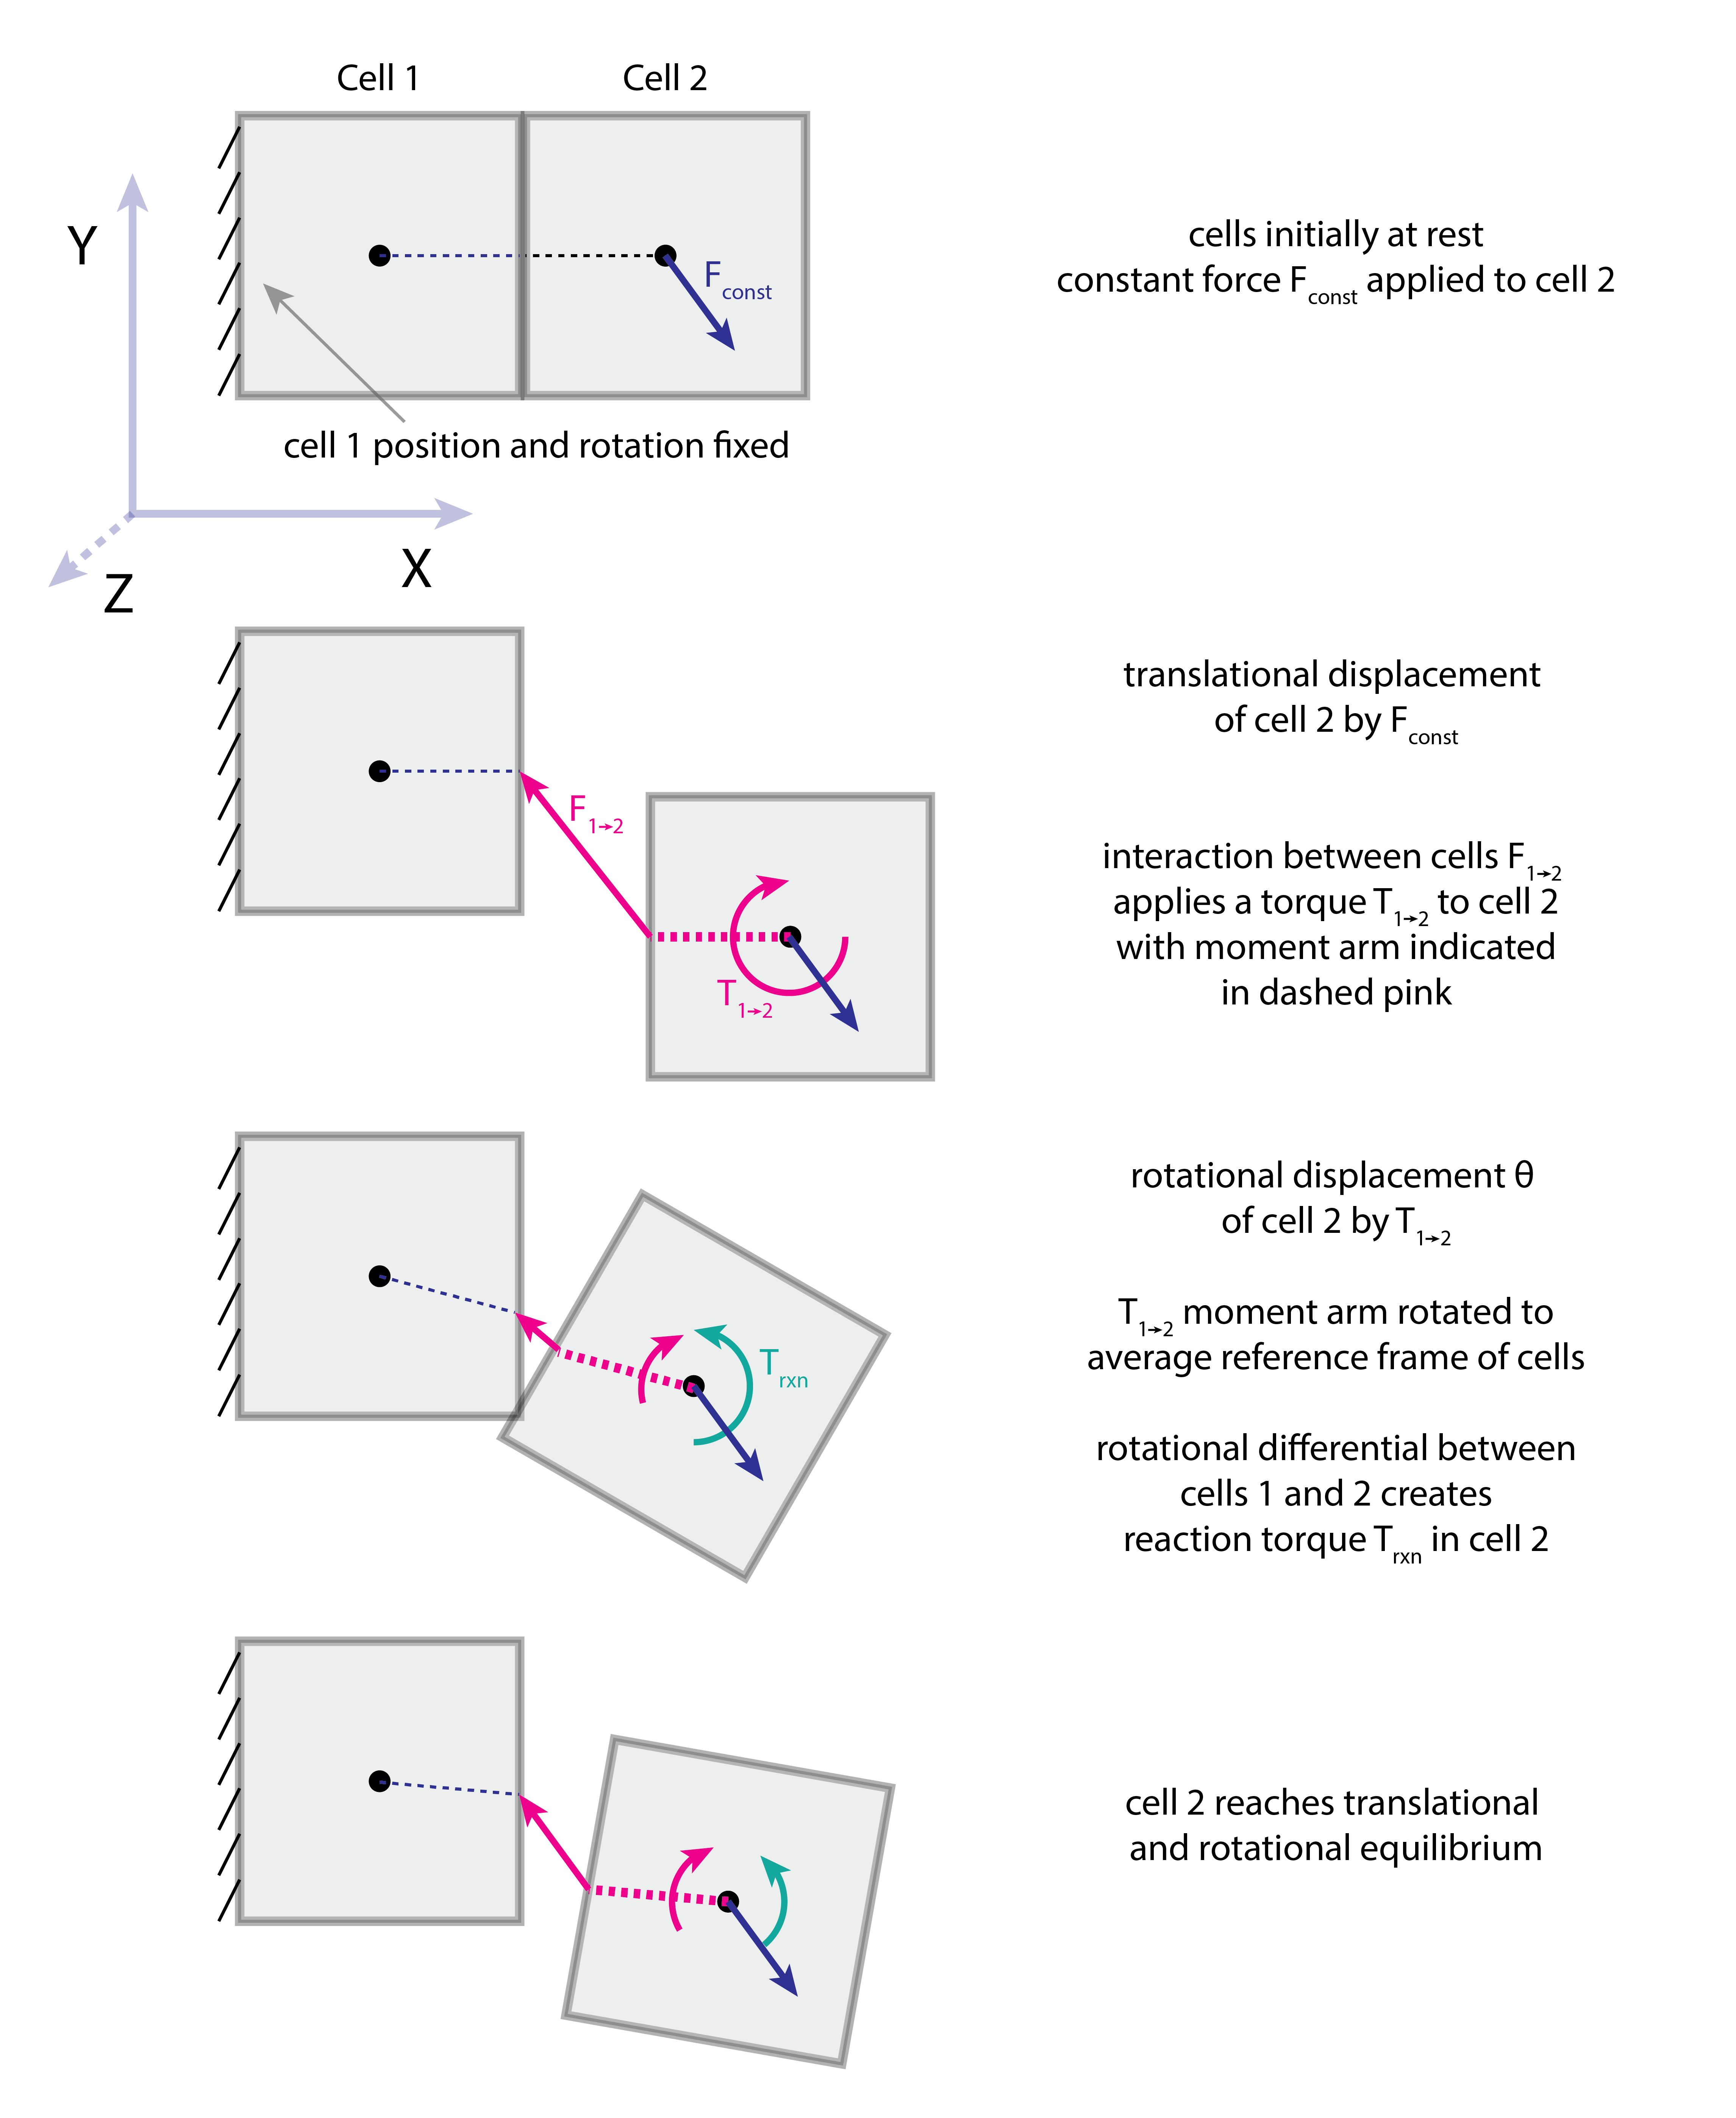
\includegraphics[width=\linewidth]{rotationalSim.png}
  \caption{rotationalSim}
  \label{fig:rotationalSim}
\end{figure}

A sketch of the translational and rotational model for cell interaction is shown in Figure \ref{fig:rotationalSim}.  In this model, we consider the fact that shear and longitudinal forces between cells are not applied directly to the center of mass of a cell, but rather at some moment arm from the center of mass.  We define the moment arm $\vec{r}_{moment2}$ of cell 2 to be half the nominal distance from cell 2 to cell 1, rotated to the average reference frame of the two cells:

\[ \vec{r}_{moment} = \dfrac{\vec{l}_{rot21}}{2}\]

Then the torque $\vec{t}_{1\rightarrow2}$ can be calculated by the cross product:

\[ \vec{t}_{1\rightarrow2} =  \vec{r}_{moment} \times \vec{f}_{1\rightarrow2}\]

If we stop now, we have set up a simulation of an arbitrary linkage of cells tied together with frictionless, spherical joints at their centers of mass.  Figure -- shows a few times steps of this system under the force of gravity.\\


\section{Sources of Error}

\begin{figure}
  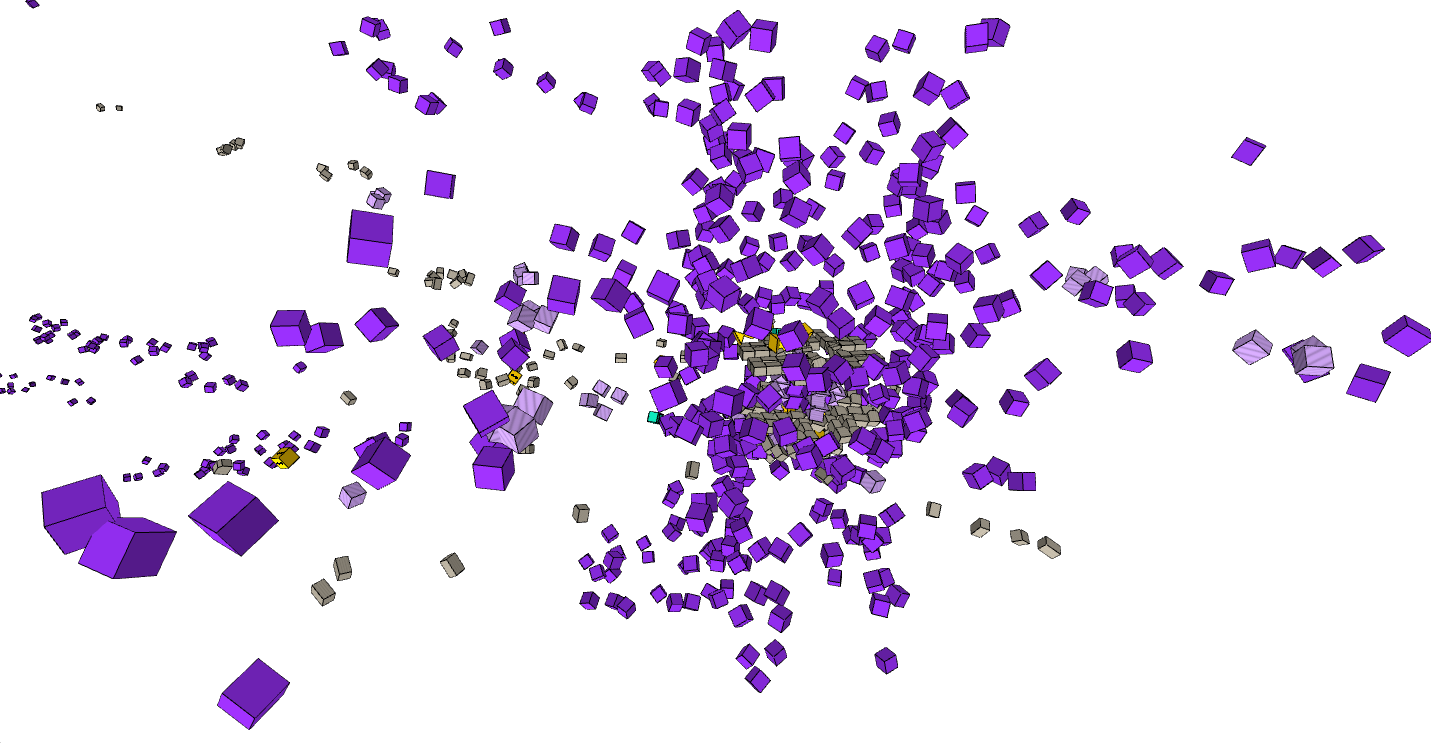
\includegraphics[width=\linewidth]{instability.png}
  \caption{instability.png.}
  \label{fig:instability}
\end{figure}

\subsection{Numerical Time Integration}

For linear systems, explicit forward time integration can be achieved using a variety of methods, each with associated error and computational cost.  The simplest and most computationally efficient approach is forward Euler:
\[ \vec{v}_{t+1} = \vec{v}_{t} +  \vec{a}_{t}\Delta t\]
\[ \vec{p}_{t+1} = \vec{p}_{t} +  \vec{v}_{t}\Delta t\]

Verlet integration requires storing the previous two position calculations (at time t and t-1) in order to calculate the next position:
\[ \vec{p}_{t+1} = 2\vec{p}_{t} - \vec{p}_{t-1} +  \vec{a}_{t}\Delta t^2\]
\[ \vec{v}_{t+1} = \dfrac{\vec{p}_{t+1} - \vec{p}_{t}}{\Delta t}\]

Higher order methods such as Runge-Kutta (RK4) reduce error further, but require multiple calculations in order to solve for a single time step.

rotational case
\[ \vec{\omega}_{t+1} = \vec{\omega}_{t} +  \vec{\alpha}_{t}\Delta t\]
\[ \dot{q} = 1/2\vec{\omega}*q\]
again, with $\vec{\omega}$ as a 4-space vector with $w=0$ and $*$ denoting the Hamilton product.

\subsection{Floating Point Operations}

\section{Electronic Simulation}\label{sec:electronicSim}

\section{Hierarchical Simulation}

\section{Performance Speedups}

A faster method of applying quaternions to vectors is given by
\[ t = 2 \left[ \begin{array}{ccc}
q_x\\
q_y\\
q_z
 \end{array} \right] \times v\]
\[ v_{rotated} = v + q_wt +  \left[ \begin{array}{ccc}
q_x\\
q_y\\
q_z
 \end{array} \right] \times t\]
 https://blog.molecular-matters.com/2013/05/24/a-faster-quaternion-vector-multiplication/


\section{Deviations from Reality}

\subsection{Volume Preservation}

Poisson's ratio $v$

\begin{figure}
  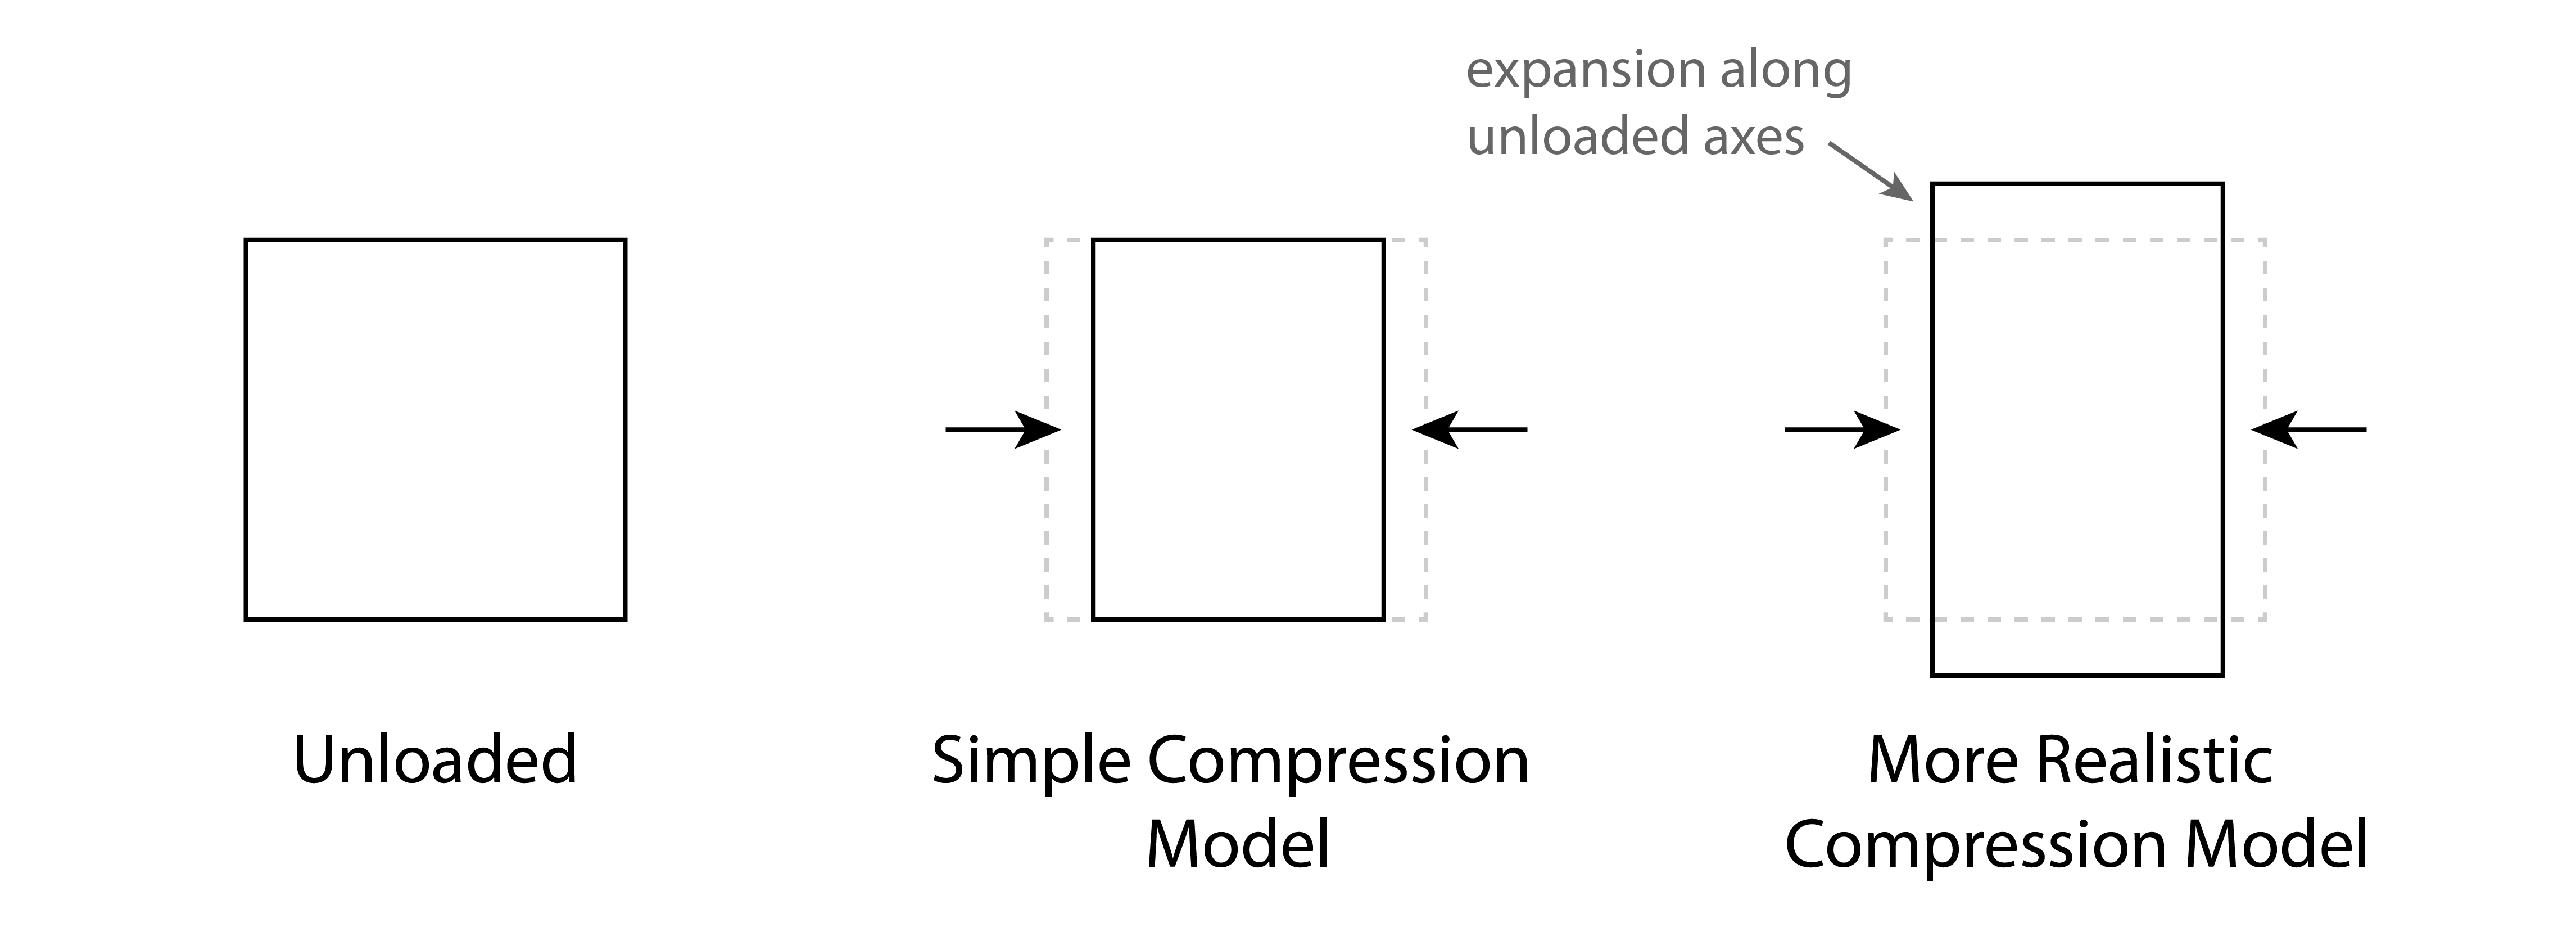
\includegraphics[width=\linewidth]{SolidMechanicsReality.png}
  \caption{Deviation from reality in simple \textit{function} simulation.  Some coupling between degrees of freedom is expected, for example, compression on one axis will result in expansion along other, unloaded axes.}
  \label{fig:SolidMechanicsReality}
\end{figure}

In reality, the degrees of freedom illustrated in Fig \ref{fig:SolidMechanicsDOF} are not completely orthogonal from one another.  For example, compression along one axis of a solid will cause some degree of expansion along the unloaded axes (Fig \ref{fig:SolidMechanicsReality}).


}
